\centerline{\bf \Huge ДЗ. Почти магические квадраты}
\centerline{\bf \Huge }

\problem{\textbf{1}} В квадрате $3 \times 3$ расставьте различные натуральные числа так, чтобы сумма чисел в каждой строке, в каждом столбце и на каждой диагонали были одинаковыми.

\begin{center}
    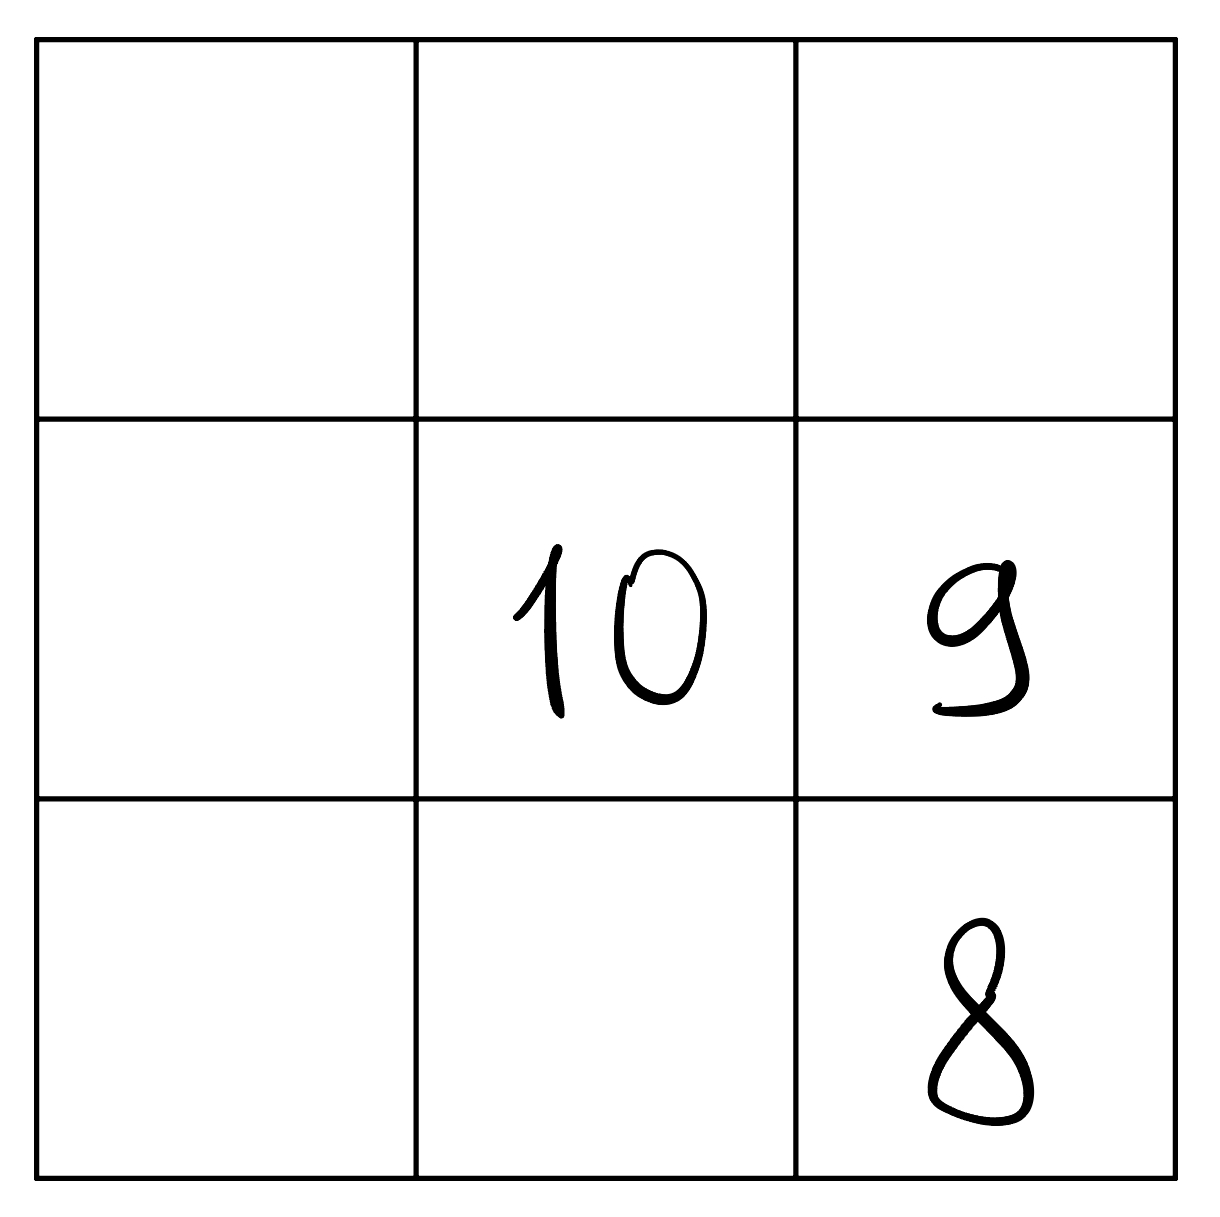
\includegraphics[width=0.2\textwidth]{ЭлМШ 2024-2025/V блок/3 и 4 группы/magic_1.png}
\end{center}


\problem{\textbf{2}} Найдите как можно больше альтернативных расстановок чисел в квадрате $3 \times 3$ из первого задания.

\problem{\textbf{3}} В квадрате $3 \times 3$ расставьте различные натуральные числа так, чтобы сумма чисел в каждой строке, в каждом столбце и на каждой диагонали были одинаковыми. 

\begin{center}
    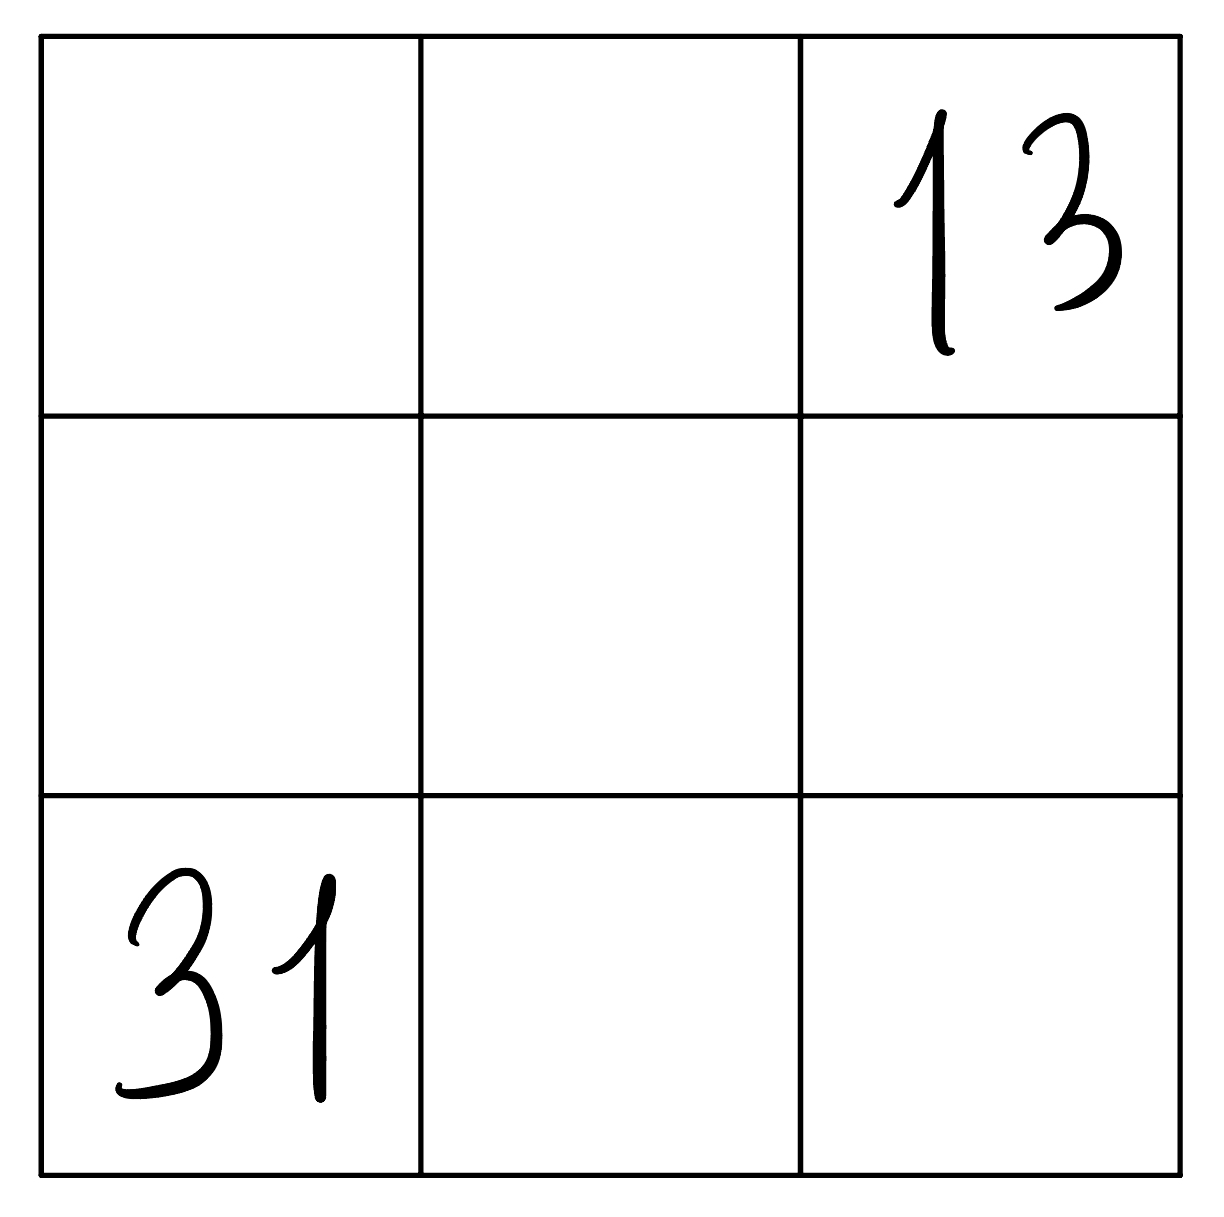
\includegraphics[width=0.2\textwidth]{ЭлМШ 2024-2025/V блок/3 и 4 группы/magic_3.png}
\end{center}

\problem{\textbf{4}} Найдите как можно больше альтернативных расстановок чисел в квадрате $3 \times 3$ из третьего задания.